\begin{frame}{Grafting: define the reaction before ranking candidates}
\large
\begin{block}{Local attachment models in acetonitrile, 298.15 K}
N--H / O--H:\quad $\mathrm{site{-}Cl + Nu{-}H \rightarrow site{-}Nu + HCl}$\\[0.8em]
N quaternization:\quad $\mathrm{site{-}Cl + Nu \rightarrow site{-}Nu^{+} + Cl^{-}}$
\end{block}
\normalsize Compare within each reaction class. An explicit base contribution is still pending.
\par\medskip\footnotesize These are capped-site thermodynamic models. Activation barriers, yields, site accessibility and polymer interactions are separate questions.
\end{frame}
\begin{frame}{Grafting thermodynamics: the first computed results}
\centering
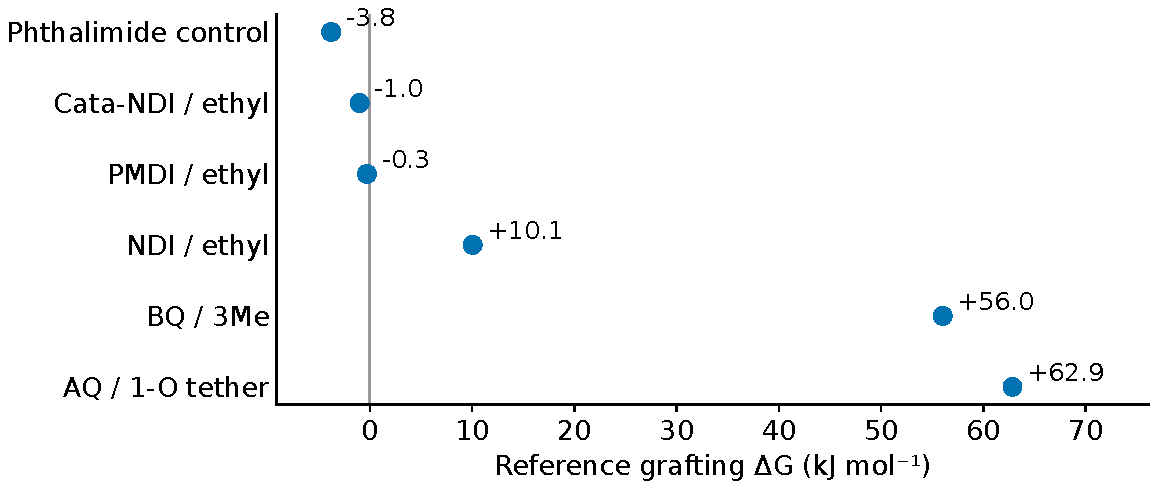
\includegraphics[width=.97\linewidth,height=.68\textheight,keepaspectratio]{../results/reviews/2026-10-19/grafting_submission/first_results/grafting_slide.pdf}
\par\smallskip\footnotesize N--H/O--H reference: $\mathrm{site{-}Cl + Nu{-}H \rightarrow site{-}Nu + HCl}$. Base capture is uncomputed; values do not predict grafting rates or yields.
\par\smallskip\scriptsize 10/75 reactions qualified at 2026-10-19 20:42 Chicago; continued calculations update the visual report.
\end{frame}
